% !TeX program = lualatex
% ================================================================
% Polish Tier 3 Vocabulary Version of ExpandingBracketsStarter
%
% Generated by the server using the following settings:
%
%   language            Polish (pol)
%   text direction      left to right
%   font                Noto Serif
%   fallback font       Noto Serif
%   built from          latex/starters/targeted/KS3/algebra/expandingBracketsStarter.tex
%   vocabulary key      latex/starters/targeted/KS3/algebra/expandingBracketsStarter/L2/pol/expandingBracketsStarter_polishKey.tex
%   tier 3 vocabulary   green   RGB 0 128 0
%   English text        black   RGB 0 0 0
%   Polish text         purple  RGB 112 48 160
%   layout macros       version 3
%
% Please don't edit any information in this comment block - the server
% compares it against the current settings and rebuilds this file when
% they differ, so changes here would be overwritten. However, feel free
% to make updates to the LaTeX below if you want to edit it.
% ================================================================

\documentclass{beamer}
% ================================================================
% Copied from the English sheet this was translated from, so that
% anything it sets up for itself still works here
% ================================================================
% Theme (optional but nice)
\usetheme{Madrid}

% Maths
\usepackage{amsmath}

% Graphics
\usepackage{tikz}

% ================================================================
% Answer-overlay helpers
% ================================================================
\newcommand{\ablank}[1]{%
  \alt<2>{\textcolor{red}{#1}}{\underline{\phantom{#1}}}%
}
\newcommand{\ashow}[1]{\uncover<2->{\textcolor{red}{\small #1}}}
\newcommand{\ashowq}[1]{\alt<2->{\textcolor{red}{\small #1}}{?}}

% Answers drawn straight on to a TikZ diagram, revealed on overlay 2 like \ashow.
% Space is reserved on overlay 1, so the diagram does not move between slides.
\usetikzlibrary{overlay-beamer-styles}
\tikzset{
  ans/.style     = {red, thick, visible on=<2->},
  ansfill/.style = {red!15, visible on=<2->},
  anslab/.style  = {red, font=\tiny, visible on=<2->},
}

% Characters this language's font has not got are borrowed from another,
% rather than being silently dropped - see docs/translated-sheet-latex.md
\directlua{%
  if luaotfload and luaotfload.add_fallback then
    luaotfload.add_fallback("eallatinfallback",
      { "Noto Serif:mode=harf;" })
  else
    tex.error("this luaotfload is too old to register a fallback font")
  end
}
\usepackage[english]{babel}
\babelprovide[import]{polish}
\babelfont[polish]{rm}[Renderer=Harfbuzz, BoldFont={Noto Serif}, ItalicFont={Noto Serif}, BoldItalicFont={Noto Serif}, RawFeature={fallback=eallatinfallback}]{Noto Serif}
\babelfont[polish]{sf}[Renderer=Harfbuzz, BoldFont={Noto Serif}, ItalicFont={Noto Serif}, BoldItalicFont={Noto Serif}, RawFeature={fallback=eallatinfallback}]{Noto Serif}
\newcommand{\ealtext}[1]{\foreignlanguage{polish}{#1}}
\newcommand{\ealtextblock}[1]{{\raggedright\foreignlanguage{polish}{#1}\par}}
% ================================================================
% EAL layout helpers
% ================================================================
\usepackage{xcolor}

\definecolor{ealkeycolour}{RGB}{0,128,0}
\definecolor{ealenglish}{RGB}{0,0,0}
\definecolor{ealtwocolour}{RGB}{112,48,160}

\newsavebox{\ealboxen}
\newsavebox{\ealboxtr}
\newlength{\ealglosswd}
\newlength{\ealglossraise}
\setlength{\ealglossraise}{1.15em}

% a tier 3 word, in English and in translation alike
\newcommand{\ealkey}[1]{\textcolor{ealkeycolour}{#1}}
\newcommand{\ealkeytr}[1]{\textcolor{ealkeycolour}{\ealtext{#1}}}

% One translated word above one English word. Built from kernel
% primitives, never a tabular, which would break wherever the sheet
% loads array, booktabs or tabularx. The box is as wide as the wider of
% the two, so a long translation pushes its neighbours aside instead of
% overlapping them, and it claims its full height so a table row or a
% TikZ node makes room for it.
\newcommand{\ealgloss}[2]{%
  \sbox{\ealboxen}{\ealkey{#1}}%
  \sbox{\ealboxtr}{\small\textcolor{ealtwocolour}{\ealtext{#2}}}%
  \setlength{\ealglosswd}{\wd\ealboxen}%
  \ifdim\wd\ealboxtr>\ealglosswd\setlength{\ealglosswd}{\wd\ealboxtr}\fi
  \leavevmode
  \makebox[\ealglosswd][c]{%
    \makebox[0pt][c]{\usebox{\ealboxen}}%
    \makebox[0pt][c]{\raisebox{\ealglossraise}{\usebox{\ealboxtr}}}%
  }%
}

% opens up line spacing around a block of glosses, so the raised
% translations sit clear of the line above
\newenvironment{ealglossed}{\par\linespread{2.1}\selectfont\ignorespaces}{\par}

% a whole translated sentence above its English counterpart. block level,
% so it does not belong inside a tabular cell
\newcommand{\ealpara}[2]{%
  \par\addvspace{0.5\baselineskip}%
  {\color{ealtwocolour}\ealtextblock{#1}}%
  \penalty200
  {\color{ealenglish}#2\par}%
  \addvspace{0.5\baselineskip}%
}

\begin{document}

\begin{frame}{Starter: Prior Knowledge}
\begin{ealglossed}
\begin{minipage}[t]{0.48\textwidth}

\begin{block}{1) \ealgloss{Arithmetic}{arytmetyka}}
\Large
\[
13 + 9 = \ablank{22}
\]
\end{block}

\vspace{6.2em}

\begin{block}{3) Collect \ealgloss{like terms}{wyrazy podobne}}
\Large
\[
3b + 4 + 2b = \ablank{5b+4}
\]
\end{block}

\end{minipage}\hfill
\begin{minipage}[t]{0.48\textwidth}

\begin{block}{2) \ealgloss{Box Method}{metoda pudełkowa}}
\centering
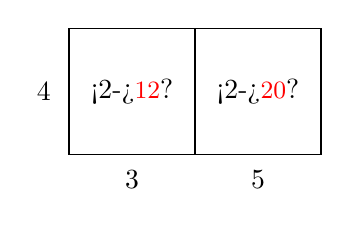
\begin{tikzpicture}[scale=0.8]

\draw (0,0) rectangle (4,2);
\draw (2,0) -- (2,2);

\node at (1,-0.4) {$3$};
\node at (3,-0.4) {$5$};
\node at (-0.4,1) {$4$};

\node at (1,1) {\ashowq{12}};
\node at (3,1) {\ashowq{20}};

\end{tikzpicture}

\vspace{0.4em}
Find the total \ealgloss{area}{pole}. \ashow{Total \ealgloss{area}{pole} $= 32$}

\end{block}

\vspace{0.6em}

\begin{block}{4) \ealgloss{Expand}{wymnażać nawiasy} the \ealgloss{bracket}{nawias}}
\Large
\[
2(x+6) = \ablank{2x+12}
\]
\end{block}

\end{minipage}
\end{ealglossed}
\end{frame}


\begin{frame}{Starter: Answers}
\begin{ealglossed}
\begin{minipage}[t]{0.48\textwidth}

\begin{block}{1) \ealgloss{Arithmetic}{arytmetyka}}
\Large
\[
13 + 9 = \textcolor{red}{22}
\]
\end{block}

\vspace{6.2em}

\begin{block}{3) Collect \ealgloss{like terms}{wyrazy podobne}}
\Large
\[
3b + 4 + 2b = \textcolor{red}{5b + 4}
\]
\end{block}

\end{minipage}\hfill
\begin{minipage}[t]{0.48\textwidth}

\begin{block}{2) \ealgloss{Box Method}{metoda pudełkowa}}
\centering
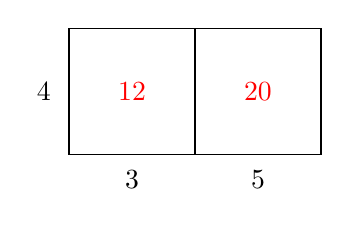
\begin{tikzpicture}[scale=0.8]

\draw (0,0) rectangle (4,2);
\draw (2,0) -- (2,2);

\node at (1,-0.4) {$3$};
\node at (3,-0.4) {$5$};
\node at (-0.4,1) {$4$};

\node at (1,1) {\textcolor{red}{12}};
\node at (3,1) {\textcolor{red}{20}};

\end{tikzpicture}

\vspace{0.4em}
\textcolor{red}{Total \ealgloss{area}{pole} = 32}

\end{block}

\vspace{0.6em}

\begin{block}{4) \ealgloss{Expand}{wymnażać nawiasy} the \ealgloss{bracket}{nawias}}
\Large
\[
2(x+6) = \textcolor{red}{2x + 12}
\]
\end{block}

\end{minipage}
\end{ealglossed}
\end{frame}

\end{document}